% !TEX root = ../notes_template.tex
\chapter{Electronics Review}\label{chp:electronics}

This chapter is a quick review of basic circuit theory and electronics. Prior knowledge of these topics is assumed, along with basic understanding of linear time invariant systems - Fourier/Laplace transforms, linear constant coefficient differential equations, transfer functions, and frequency response. The reader is encouraged to review the material in this chapter before proceeding to the next chapter.

\section{Review of Basic Circuit Theory}
The interaction of electromagnetic fields with matters is the basis of all electrical and electronic devices. These interactions are often described, analyzed and synthesized through the abstractions of electrical circuit theory. The following are the most basic circuit two-terminal elements we will need for now. We will introduce new ones as and when they are required. Each circuit element has a unique voltage-current relationship, and it is \emph{important} that you know these by heart.

\begin{figure}[b]
    \centering
    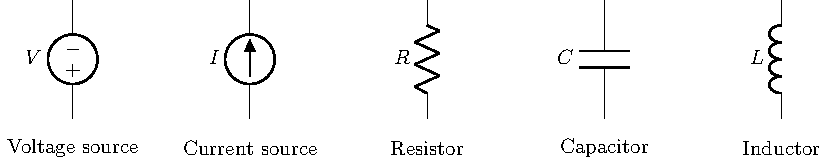
\includegraphics[width=\textwidth]{figure/fig02-01.pdf}
    \caption{Basic circuit elements: voltage source, current source, resistor, capacitor, and inductor.}
    \label{fig:02-01}
\end{figure}

\noindent\textbf{Voltage source.} An idea voltage source provides a fixed voltage $V$ between its two terminals, and can provide any amount of current. Notice that the voltage $V$ can be fixed or time varying. For example, for a DC vortlage source with $V = 5V$, the voltage across the two terminals will be $5V$ for all time. But for a time varying AC source, $V = 5 \sin \left( 100\pi t \right)$, the voltage across its terminal will vary with time.

\noindent \textbf{Current source.} An ideal cuyrrent source provide a fixed amount of current to flow throgh its terminals (out through one and in through the other), irrespective of the voltage across its terminals. Current sources can also be time-varying.

\noindent \textbf{Resistor.} A passive element where the current $i_R$ flowing through the element is proportional to the voltage $v_R$ across its terminals.
\[ v_R \propto i_R \]
In the case of linear resistors, the proportionality factor is constant, resulting in Ohm's law,
\begin{equation}
    v_R = R \, i_R
    \label{eq:ch02-01}
\end{equation}

The units of $R$ are $V.A^{-1}$ or $Omhs \left( \Omega \right)$. $R$ is in general positive. The power absorbed by a resistor is given by the product of the voltage across it and the current flowing through the resistor, 
\begin{equation}
    P = v_R \, i_R = i_R^2 \, R = \frac{v_R^2}{R}
    \label{eq:ch02-02}
\end{equation}
This power is dissipated as heat by the resistor. Note that the power absorbed by a resistor is always positive, since $R$ is positive.

We will later see non-linear resistors, where the resistance varies as a function of the applied votlage, temperature and other factors. 

\noindent \textbf{Capacitor.} A capacitor is another passive element with the following voltage current relationship.
\begin{equation}
    i_C = C \frac{d v_C}{dt}
    \label{eq:ch02-03}
\end{equation}

The current $i_C$ through the capacitor is proportional to the rate of change of voltage across its terminals $v_C$. The proportionality factor is called the capacitance $C$, and has units of $F$ (Farads) or $C \cdot V^{-1}$. The voltage across the capacitor is given by at any given time is proportional to the integral of the current flowing through itor the charge stored in the capacitor. The voltage across the capacitor is given by
\begin{equation}
    q = C \, v_C
    \label{eq:ch02-04}
\end{equation}

The instantaneous power absorbed by the capacitor is given by,
\begin{equation}
    P = v_C \, i_C = C \, v_C \frac{d v_C}{dt}
    \label{eq:ch02-05}
\end{equation}

The power absorbed by the capacitor can be positive or negative, depending on the direction of current flow. If the current is flowing into the capacitor, then the voltage across it is increasing, and the power absorbed is positive. If the current is flowing out of the capacitor, then the voltage across it is decreasing, and the power absorbed is negative. A capacitor stores energy in the electric field between its plates. The energy stored in a capacitance at any given time depends on the charge stored in it, and is given by,
\begin{equation}
    E = \frac{1}{2}  C \, v_C^2
    \label{eq:ch02-06}
\end{equation}

\noindent \textbf{Inductor.} An inductor is another passive element with the following voltage current relationship.
\begin{equation}
    v_L = L \frac{di_L}{dt}
    \label{eq:ch02-07}
\end{equation}

The voltage $v_L$ across the inductor is proportional to the rate of change of current $i_L$ flowing through it. The proportionality factor is called the inductance $L$, and has units of $H$ (Henries) or $V \cdot s \cdot A^{-1}$. The current through the inductor is given by at any given time is proportional to the integral of the voltage across it. The current through the inductor is given by
\begin{equation}
    i_L = \frac{1}{L} \int v_L \, dt
    \label{eq:ch02-08}
\end{equation}

The instantaneous power absorbed by the inductor is given by,
\begin{equation}
    P = v_L \, i_L = L \, i_L \frac{di_L}{dt}
    \label{eq:ch02-09}
\end{equation}

The power absorbed by the inductor can be positive or negative, depending on the direction of current flow. If the current is flowing into the inductor, then the voltage across it is increasing, and the power absorbed is positive. If the current is flowing out of the inductor, then the voltage across it is decreasing, and the power absorbed is negative. An inductor stores energy in the magnetic field around it. The energy stored in an inductor at any given time depends on the current flowing through it, and is given by,
\begin{equation}
    E = \frac{1}{2}  L \, i_L^2
    \label{eq:ch02-10}
\end{equation}

\subsection{Kirchoff's Laws}
The five elements alone are not that interesting. But interesting things can be done by connecting these elements together in different ways to form an electrical circuit. The elements are connected together by wires, whicha are assumed to be perfect conductors, i.e. zero resistance. Consider the following circuit (Figure \ref{fig:02-01}),
\begin{figure}[t]
    \centering
    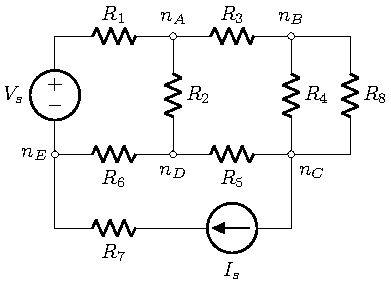
\includegraphics[width=0.5\textwidth]{figure/fig02-02.pdf}
    \caption{A simple electrical circuit with a voltage sourse, a current source, and a bunch of resistors.}
    \label{fig:02-02}
\end{figure}

How do we find out the voltages and currents in the circuit? Kirchoff's laws can be used for analysing such circuits, which are based on the conservation of charge and energy. The circuit in Figure \ref{fig:02-02} is a simple electrical circuit with a voltage source, a current source, and a bunch of resistors. The voltage source provides a fixed voltage $V_s$ between its two terminals, and the current source provides a fixed amount of current $I_s$ to flow through its terminals. The voltages and currents in the rest of the elements will be determined by Kirchoff's laws with the constraints imposed by the voltage and current sources. The two laws are:

\begin{enumerate}
    \item \textbf{Kirchoff's current law (KCL):} The sum of the currents entering a node is equal to the sum of the currents leaving the node. A \textit{node} is a point at which two or more circuit elements are connected together. In Figure \ref{fig:02-02}, $n_A$, $n_B$, $n_C$ and $n_D$ are examples of nodes where three elements are connected together. There are three other nodes in the circuit, can you identify them? 
    
    The sum of the currents at a node is equal to zero. This is based on the conservation of charge, and can be expressed mathematically as:
    \begin{equation}
        \sum_{i=1}^{n} i_i = 0
        \label{eq:ch02-11}
    \end{equation}
    where $i_i$ is the current flowing into or out of the node, and $n$ is the number of elements connected to the node. The current flowing into a node is positive, and the current flowing out of a node is negative.
    
    \item \textbf{Kirchoff's voltage law (KVL):} The sum of the voltages around a closed loop in a circuit is equal to zero. A \textit{closed loop} is a path in the circuit that starts and ends at the same node, and does not cross itself. In Figure \ref{fig:02-02}, the path starting from $n_A$, to $n_D$, to $n_B$, and back to $n_A$ is a closed path. This path invludes the resistors $R_3$, $R_4$, $R_5$, and $R_2$. 
    
    This is based on the conservation of energy, and can be expressed mathematically as:
    \begin{equation}
        \sum_{i=1}^{n} v_i = 0
        \label{eq:ch02-12}
    \end{equation}
    where $v_i$ is the voltage across each element in the loop, and $n$ is the number of elements in the loop.

    The voltage across an element is positive if the current is flowing into the positive terminal of the element, and negative if the current is flowing out of the positive terminal of the element.
\end{enumerate}

Note that the two laws apply for any type of circuit element used in the circuits, independnet or dependent voltage/current sources, resistors, capacitors, inductors, other two, three or four terminal elements.

\subsection{Series and Parallel Connections}
Two elements that share the same voltage across them between a given pair of notes are said to be \textbf{parallel} to each other. In Figure~\ref{fig:02-02}, $R_4$ and $R_8$ are parallel to each other. In a single loop, two elements that share the same current are said to be in \textbf{series} with each other. In Figure~\ref{fig:02-02}, $V_s$ and $R_1$ are in series, $I_s$ and $R_7$ are in series.

\subsubsection{Resistors in series and parallel}
When $n$ resistors $R_1, R_2, \cdots R_n \geq 0$ are in series, these can be combined to an equivalent resistor with resistance $R_{eq}$ given by the following,
\begin{equation}
    R_{eq} = \sum_{i=1}^{n} R_i \implies R_{eq} \geq \max_{1 \leq i \leq n} R_i.
    \label{eq:02-13}
\end{equation}
Note that in a series connection the equivalent resistance is at least as large as the largest value of $R_1$ to $R_n$.

When $n$ resistors $R_1, R_2, \cdots R_n \geq 0$ are in parallel, these can be combined to an equivalent resistor with resistance $R_{eq}$ given by the following,
\begin{equation}
    \frac{1}{R_{eq}} = \sum_{i=1}^{n} \frac{1}{R_i} \implies R_{eq} = \frac{R_1R_2\cdots R_n}{R_1 + R_2 + \cdots + R_n} \implies R_{eq} \leq \min_{1 \leq i \leq n} R_i
    \label{eq:02-14}
\end{equation}
Note that in a parallel connection, the equivalent resistance cannot be larger than the smallest value of $R_1$ to $R_n$.

\subsubsection{Capacitors in series and parallel}
\noindent\textbf{Series connection} of $n$ capacitors $C_1, C_2, \cdots C_n \geq 0$
\begin{equation}
    C_{eq} = \frac{C_1C_2\cdots C_n}{C_1 + C_2 + \cdots + C_n}
    \label{eq:02-15}
\end{equation}

\noindent\textbf{Parallel connection} of $n$ capacitors $C_1, C_2, \cdots C_n \geq 0$
\begin{equation}
    C_{eq} = C_1 + C_2 + \cdots + C_n
    \label{eq:02-16}
\end{equation}

\subsubsection{Inductors in series and parallel}
\noindent\textbf{Series connection} of $n$ capacitors $L_1, L_2, \cdots L_n \geq 0$
\begin{equation}
    L_{eq} = L_1 + L_2 + \cdots + L_n
    \label{eq:02-17}
\end{equation}

\noindent\textbf{Parallel connection} of $n$ capacitors $L_1, L_2, \cdots L_n \geq 0$
\begin{equation}
    L_{eq} = \frac{L_1L_2\cdots L_n}{L_1 + L_2 + \cdots + L_n}
    \label{eq:02-18}
\end{equation}
Its left as an exercise for you to verify these expressions.

\noindent\textbf{What does the equivalent resistance actually mean?} The equilvant resistor with resistance $R_{eq}$ has the same voltage-current relationship as the individual elements in series or parallel connection. We can replace the series or parallel connection of the individual resistors $R_1$ to $R_n$ by a single resistor with value $R_{eq}$ without changing the volatage current relationships in the circuit. The same argument applies for equivalent capacitors and inductors.

% \begin{tikzpicture}
%     \draw (2.5, 0) node [npn] (t) {$Q_1$};
%     \draw (0, 0) node[ocirc] {} to[R, l=$R_1$] (t.base);
%     \draw (t.collector) to[R, l=$R_2$] ++(0, 2) -- ++(1.5, 0) node[ocirc] (p1){};
%     \draw (t.collector) node[circ] {} -- ++(1.5, 0) node[ocirc] (p2) {};
%     \draw (t.emitter) -- ++(0, -1) node[circ] (e){} -- ++ (1.5, 0) node[ocirc] (p3) {};
%     \draw (e.center) -- ++(-2.5, 0) node[ocirc]{};
%     \draw [-latex] ([xshift=-2mm]0, 0) -- ++(0, -1.8) node[midway, left] {$U_1$};
%     \draw [-latex] ([xshift=2mm]p2.center) -- ([xshift=2mm]p3.center) node[midway, left] {$U_3$};
%     \draw (t.base) node [above] {B};
%     \draw (t.collector) node [left] {C};
%     \draw (t.emitter) node [left] {E};
% \end{tikzpicture}
